\documentclass{report}
\usepackage[utf8]{inputenc}
\usepackage[italian]{babel}

\title{
    Easy Notes \\
    \large Applicazioni e Servizi Web
}

\author{Emanuele Sanchi - 0000000000 \{emanuele.sanchi@studio.unibo.it\} \\
Francesco Buda - 0000000000 \{francesco.buda3@studio.unibo.it\} \\
Tommaso Severi - 0001172431 \{tommaso.severi2@studio.unibo.it\}}
\date{\today}

\usepackage{natbib}
\usepackage{graphicx}

\begin{document}
\maketitle

\clearpage
\tableofcontents
\clearpage

\chapter{Introduzione}
\textbf{Easy Notes} è un progetto che nasce dalle reali necessità di noi studenti che,
ormai in fondo alla nostra carriera universitaria, abbiamo raccolto con l'esperienza. \\
Il progetto consiste in una semplice Web App che simula un quaderno digitale dove poter
prendere appunti direttamente in relazione alle slide delle lezioni, comunemente utilizzate
in ambito universitario. \\
Infatti, la funzionalità principale del sistema è avere, per ogni
pagina di slide, una pagina dedicata agli appunti che l'utente può prendere liberamente.
Ogni blocco di appunti può essere poi salvato direttamente insieme alle relative slide sul cloud. \\
Inoltre, anche i professori possono registrarsi al sistema per poter creare le loro classi in 
formato digitale dove caricare le slide del corso, in modo che gli utenti possano facilmente
caricarle per prenderci appunti in un'unica piattaforma. Ogni studente può poi iscriversi al corso
per poter essere notificato quando il professore carica nuovo materiale didattico. \\
Infine, il sistema prevede anche una funzionalità di riassunto automatico degli appunti presi,
tramite intelligenza artificiale, in modo da facilitare lo studio in vista degli esami. \\
In questo report verranno descritte le varie fasi di sviluppo del progetto, dalle
scelte tecnologiche al design dell'architettura, fino al deployment della Web App.
\newpage

\section{Requisiti}
Descrizione delle caratteristiche e funzionalità che il sistema prevede.

\chapter{Design}
Design dell'architettura del sistema e delle interfacce utente.

\section{Mockup}
Una parte estensiva del design si è concentrata sulla progettazione dell'interfaccia utente. 
Infatti, era cruciale dal punto di vista della nostra app che tutte le funzionalità offerte 
fossero facilmente accessibili e utilizzabili dagli utenti finali. 
Per questo motivo, la pagine principale in Figura \ref{fig:mockup_home} dell'applicazione è 
molto dettagliata e contiene al suo interno tutte le funzionalità principali dell'applicazione.
Come si può notare, la pagina è divisa a metà fra slides e note, una per pagina. Per il 
pdf sono presenti tutti i comandi per navigare o modificare il documento. Nella parte alta
sono presenti i comandi per la gestione delle note, come l'aggiunta, la modifica e la
cancellazione, nonché la possibilità di cercare per una parola chiave all'intero delle pagine. \\

\begin{figure}[h!]
    \centering
    
\includegraphics[width=1\textwidth]{mockup/Home.png}
    \caption{Mockup pagina home}
    \label{fig:mockup_home}
\end{figure}

Dal menù di navigazione in Figura \ref{fig:mockup_menu} è possibile accedere alle altre pagine
dell'applicazione:
\begin{itemize}
    \item Home, la pagina principale dell'applicazione.
    \item Notes in Figura \ref{fig:mockup_notes}, la pagina dove l'utente può visualizzare tutte le note salvate insieme
    alle slides in un unico elenco.
    \item Classes, la pagina dove l'utente può visualizzare tutte le classi a cui partecipa.
    Cambia aspetto a seconda del ruolo dell'utente:
    \begin{itemize}
        \item Figura \ref{fig:mockup_classes_student} mostra l'aspetto per gli studenti, 
        che possono solo visualizzare le classi, iscriversi e caricare le slide.
        \item Figura \ref{fig:mockup_classes_teacher} mostra l'aspetto per i docenti,
        che possono anche creare nuove classi e aggiungere le slide.
    \end{itemize}
    \item Profile in Figura \ref{fig:mockup_profile}, la pagina dove l'utente può visualizzare e modificare le 
    informazioni del proprio profilo.
\end{itemize}

\begin{figure}[h!]
    \centering
    
\includegraphics[width=1\textwidth]{mockup/Menu.png}
    \caption{Mockup menù di navigazione}
    \label{fig:mockup_menu}
\end{figure}

\begin{figure}[h!]
    \centering
    
\includegraphics[width=1\textwidth]{mockup/Notes.png}
    \caption{Mockup pagina delle note}
    \label{fig:mockup_notes}
\end{figure}

\begin{figure}[h!]
    \centering
    
\includegraphics[width=1\textwidth]{mockup/Classes Student.png}
    \caption{Mockup pagina delle classi - studente}
    \label{fig:mockup_classes_student}
\end{figure}

\begin{figure}[h!]
    \centering
    
\includegraphics[width=1\textwidth]{mockup/Classes Teacher.png}
    \caption{Mockup pagina delle classi - docente}
    \label{fig:mockup_classes_teacher}
\end{figure}

\begin{figure}[h!]
    \centering
    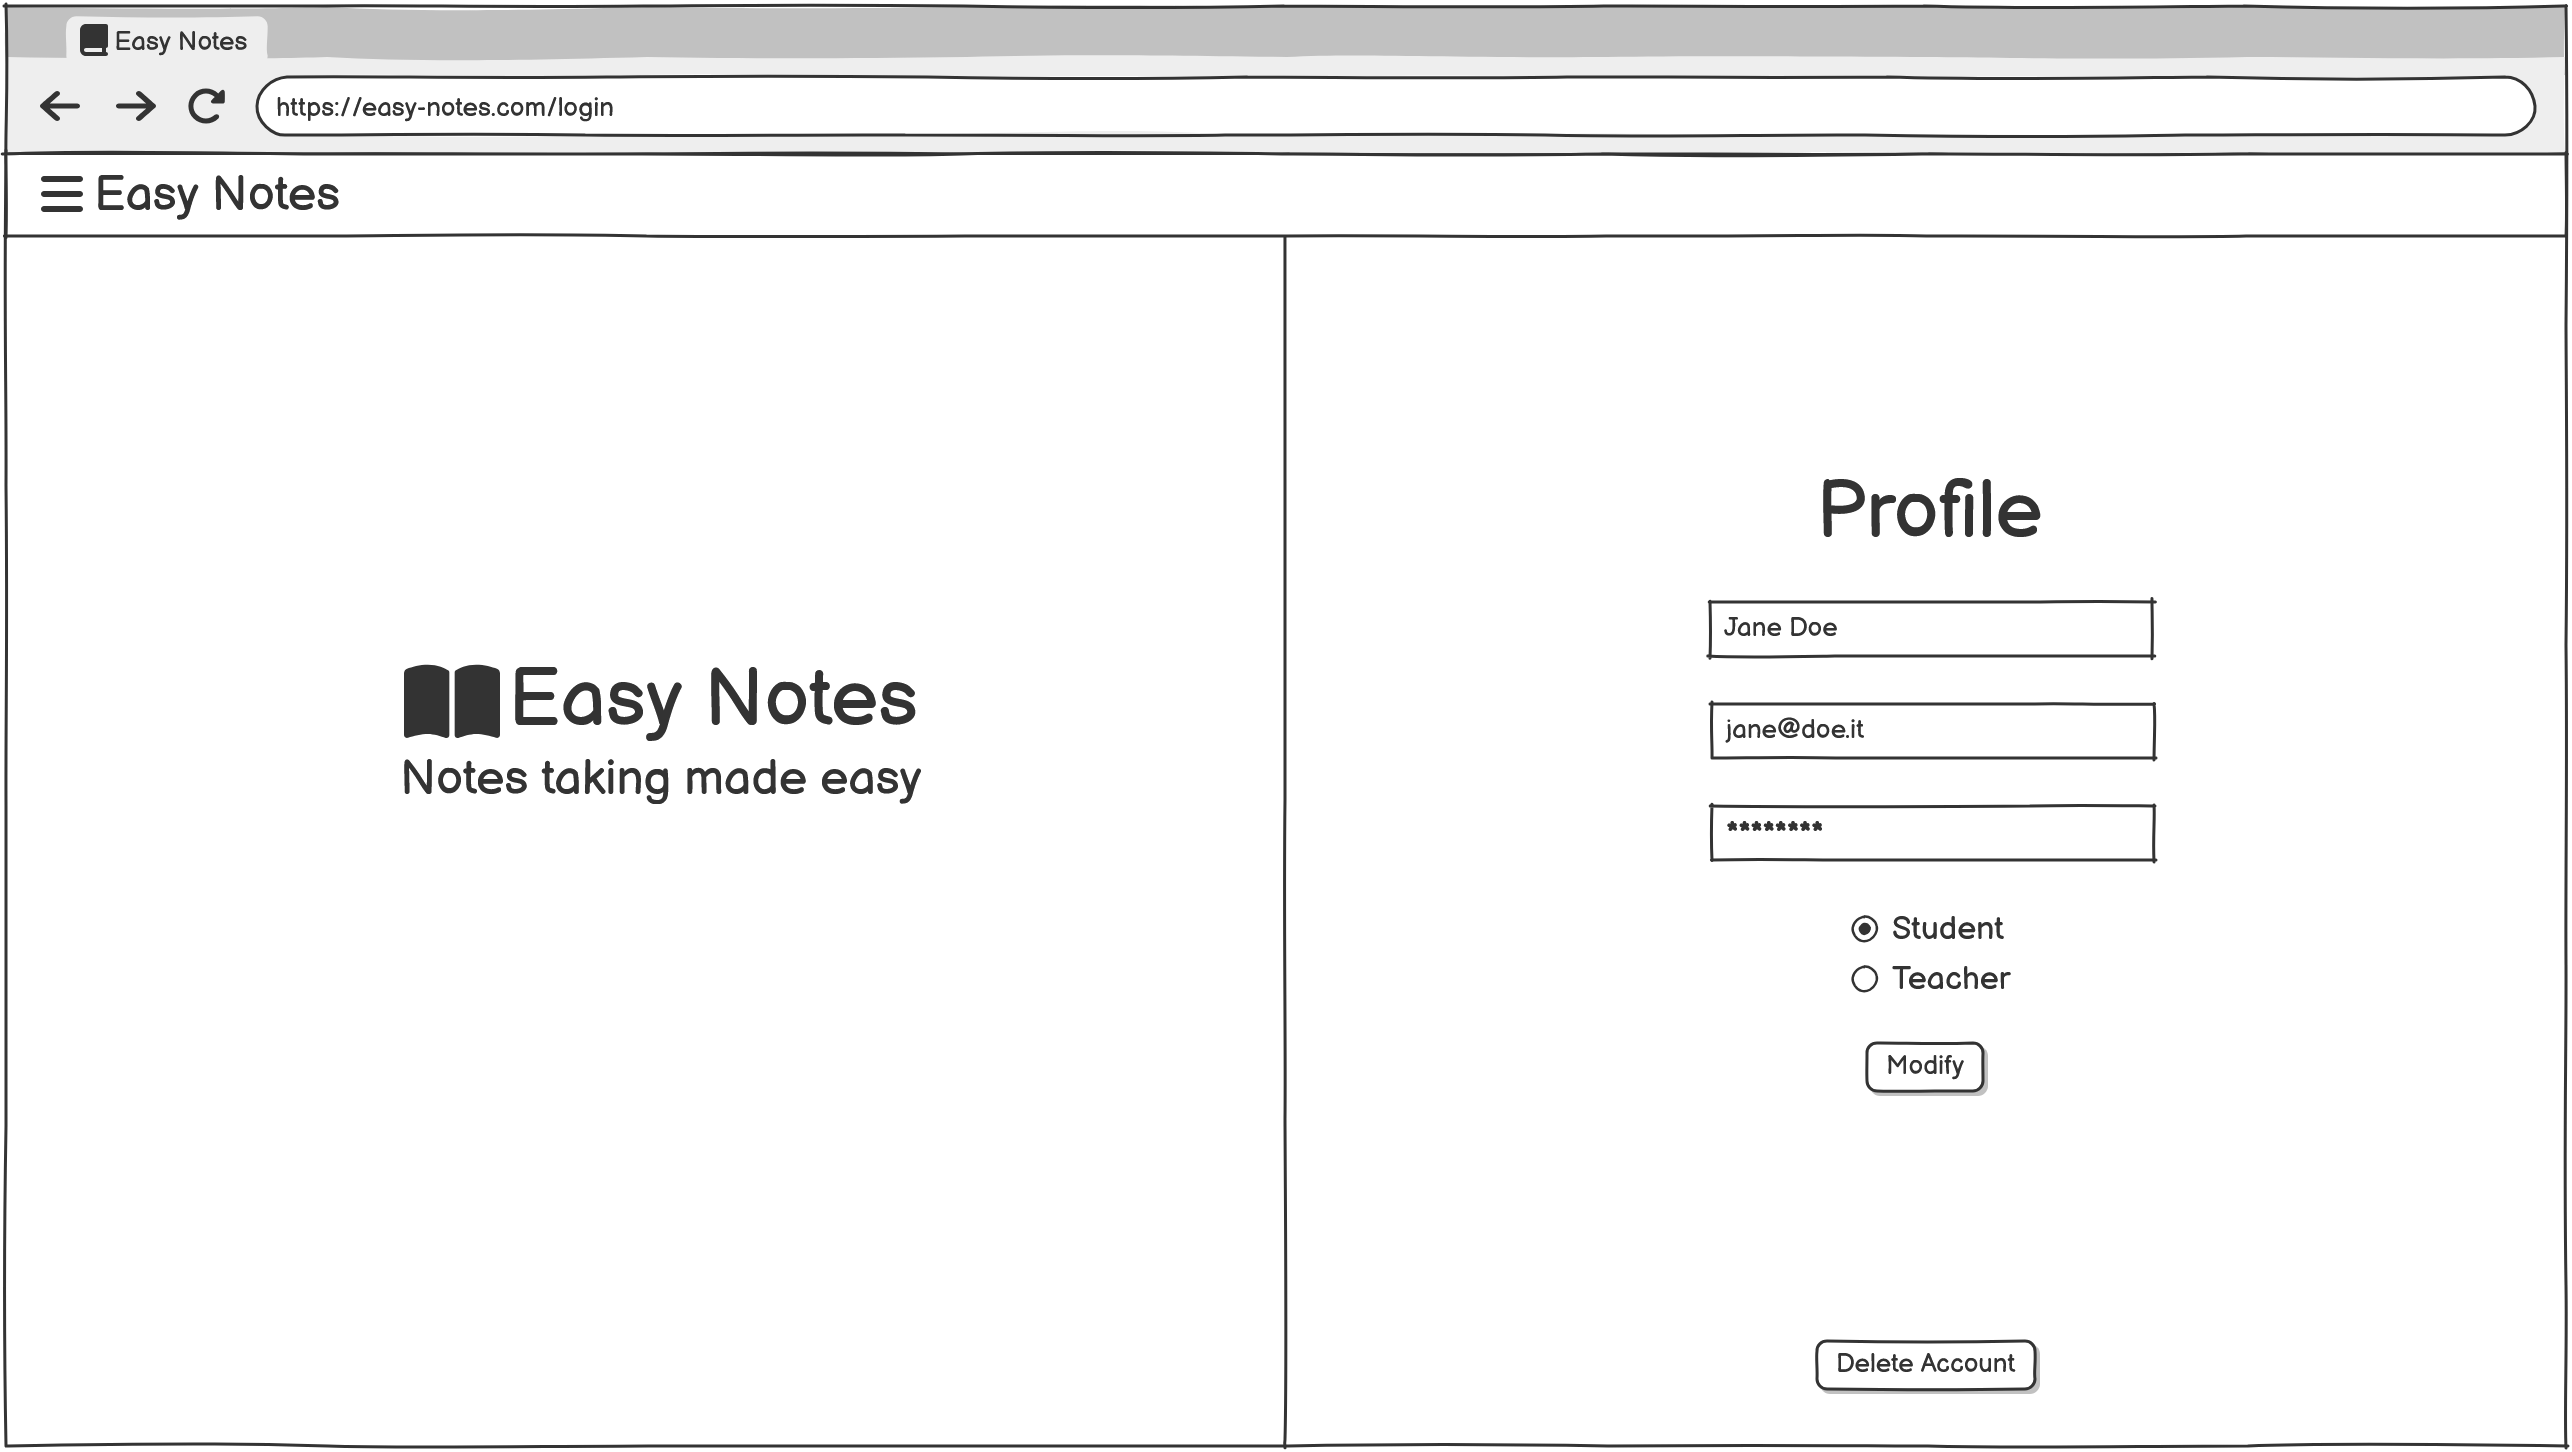
\includegraphics[width=1\textwidth]{mockup/Profile.png}
    \caption{Mockup pagina del profilo}
    \label{fig:mockup_profile}
\end{figure}

Ogni pagina all'infuori della Home necessita di un account per essere visualizzata.
Per questo motivo, la pagina di login in Figura \ref{fig:mockup_login} permette agli utenti
di autenticarsi all'applicazione. \\
La figura \ref{fig:mockup_signin} mostra invece la pagina di registrazione, dove l'utente
può creare un nuovo account inserendo le proprie informazioni personali. È in questo
momento che l'utente sceglie il proprio ruolo, che può essere studente o docente. \\

\begin{figure}[h!]
    \centering
    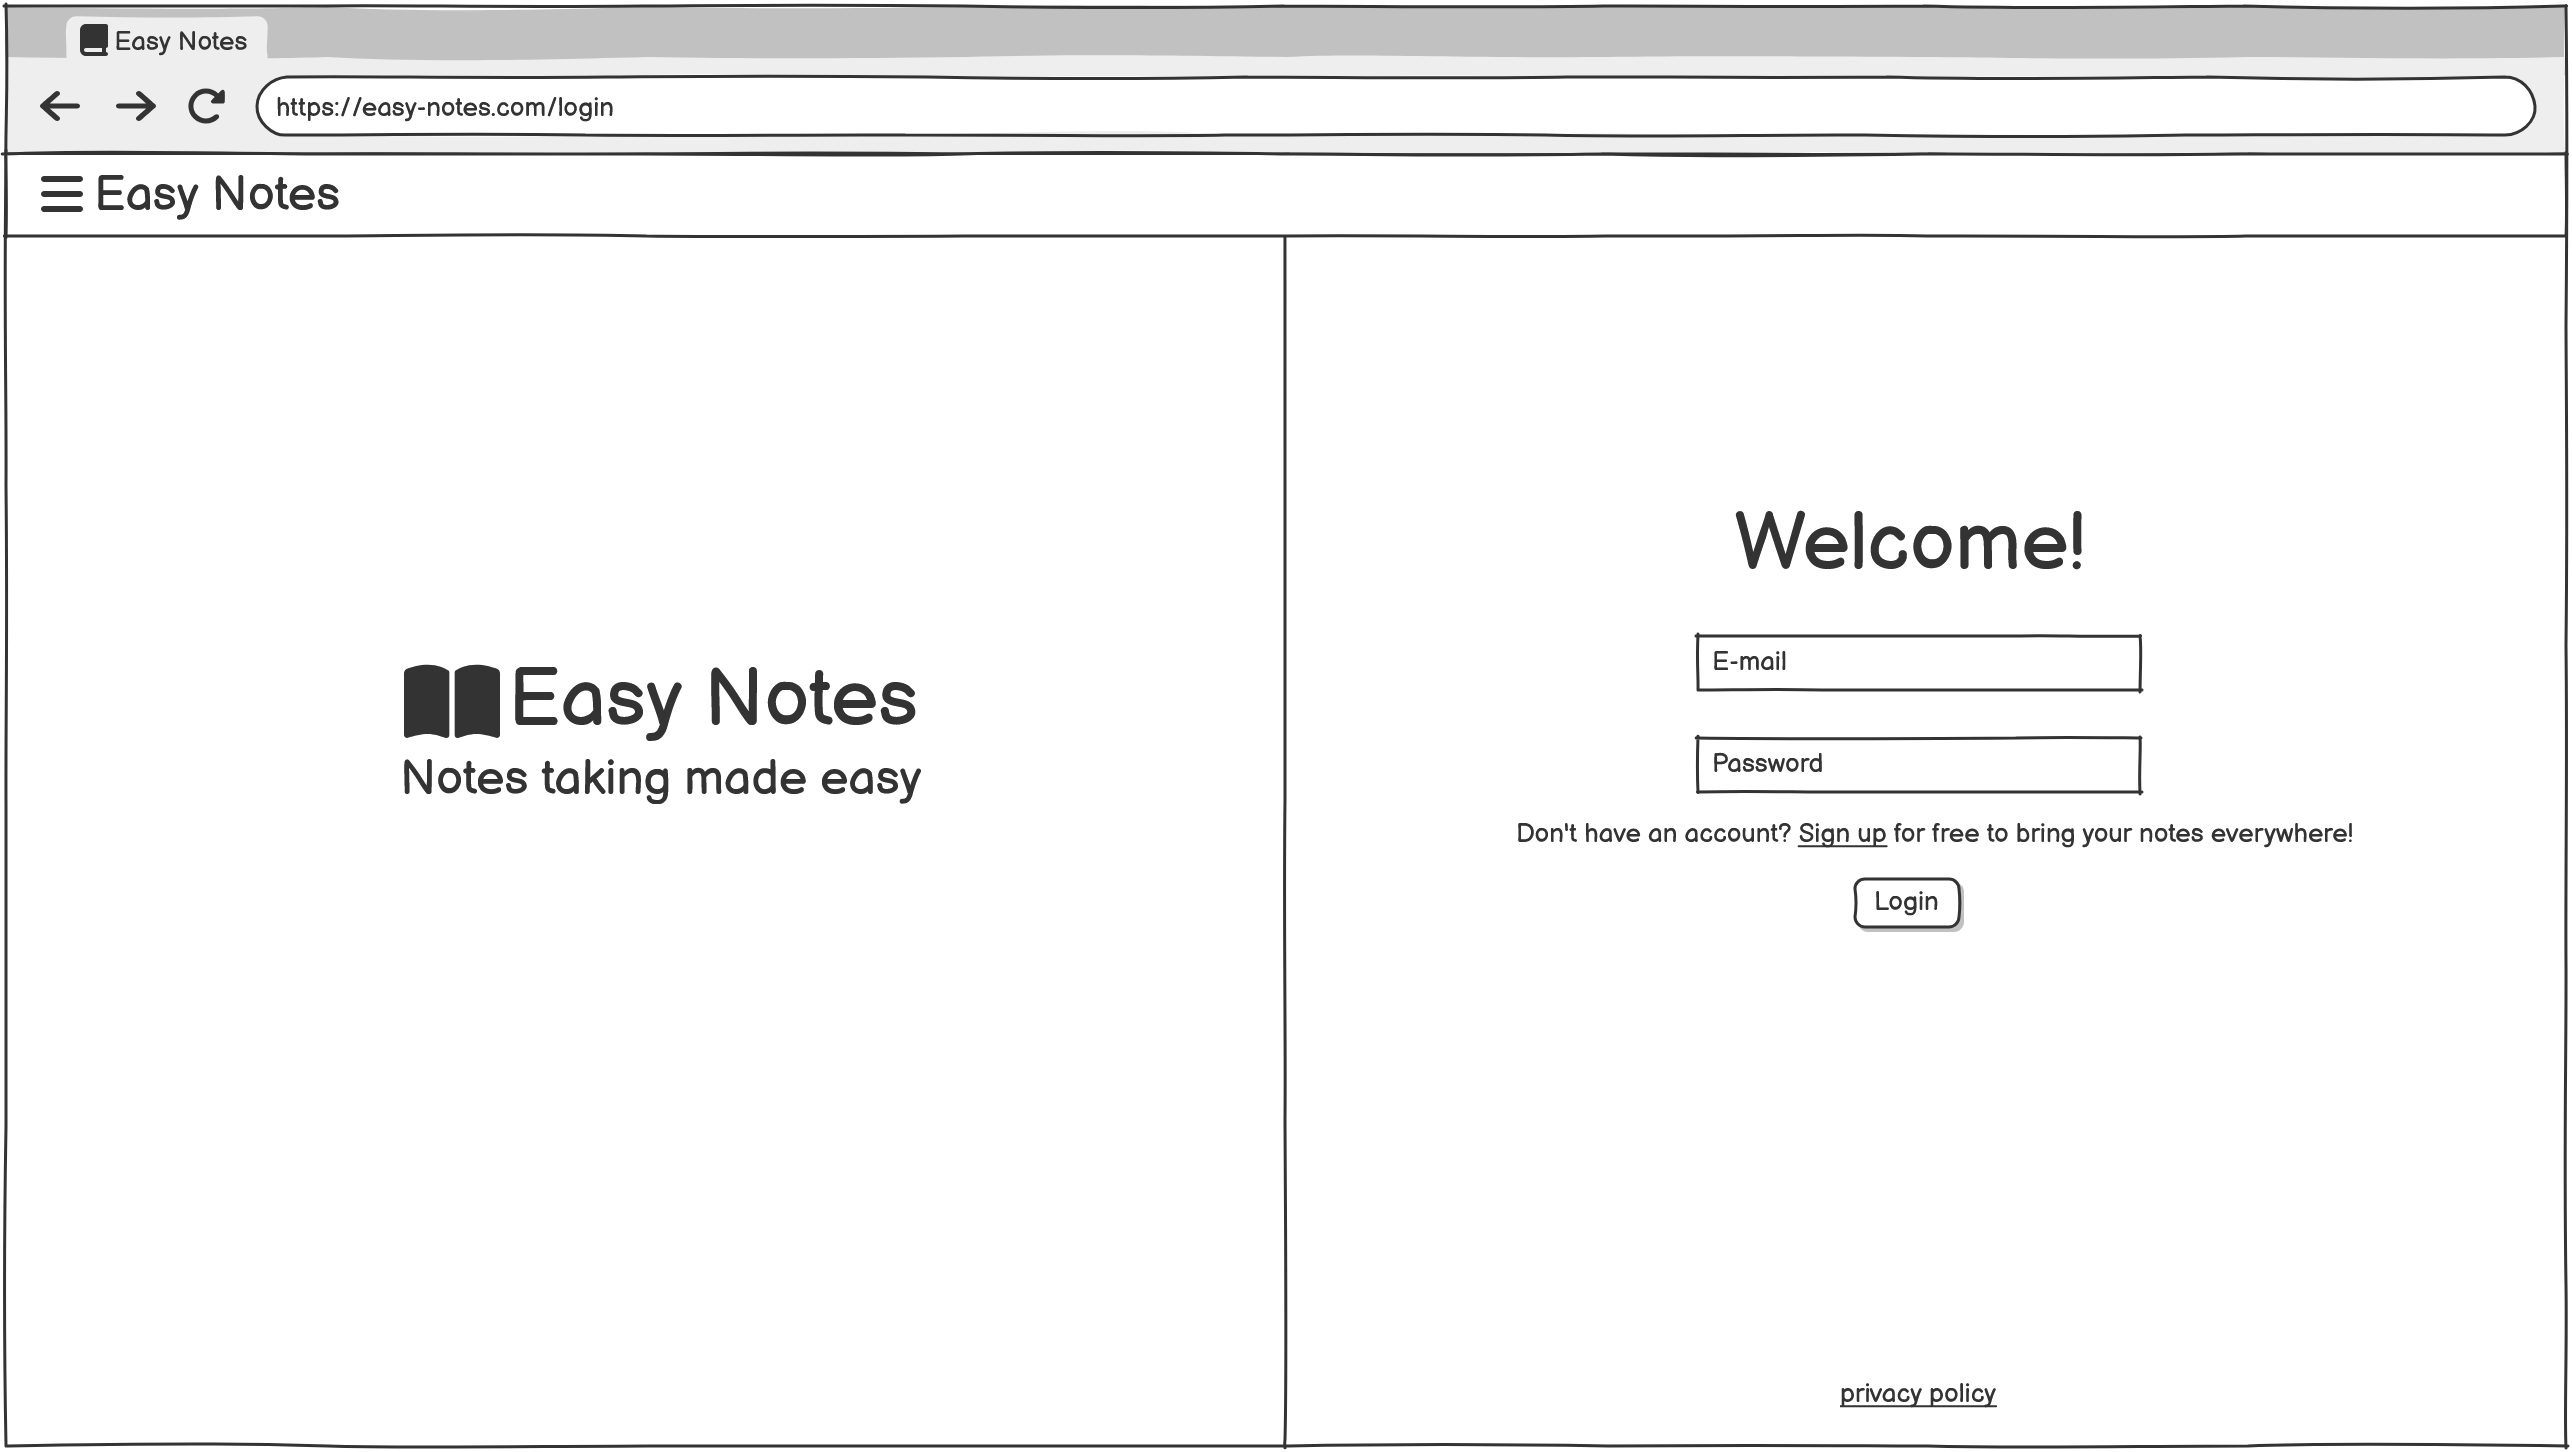
\includegraphics[width=1\textwidth]{mockup/Login.png}
    \caption{Mockup pagina di login}
    \label{fig:mockup_login}
\end{figure}

\begin{figure}[h!]
    \centering
    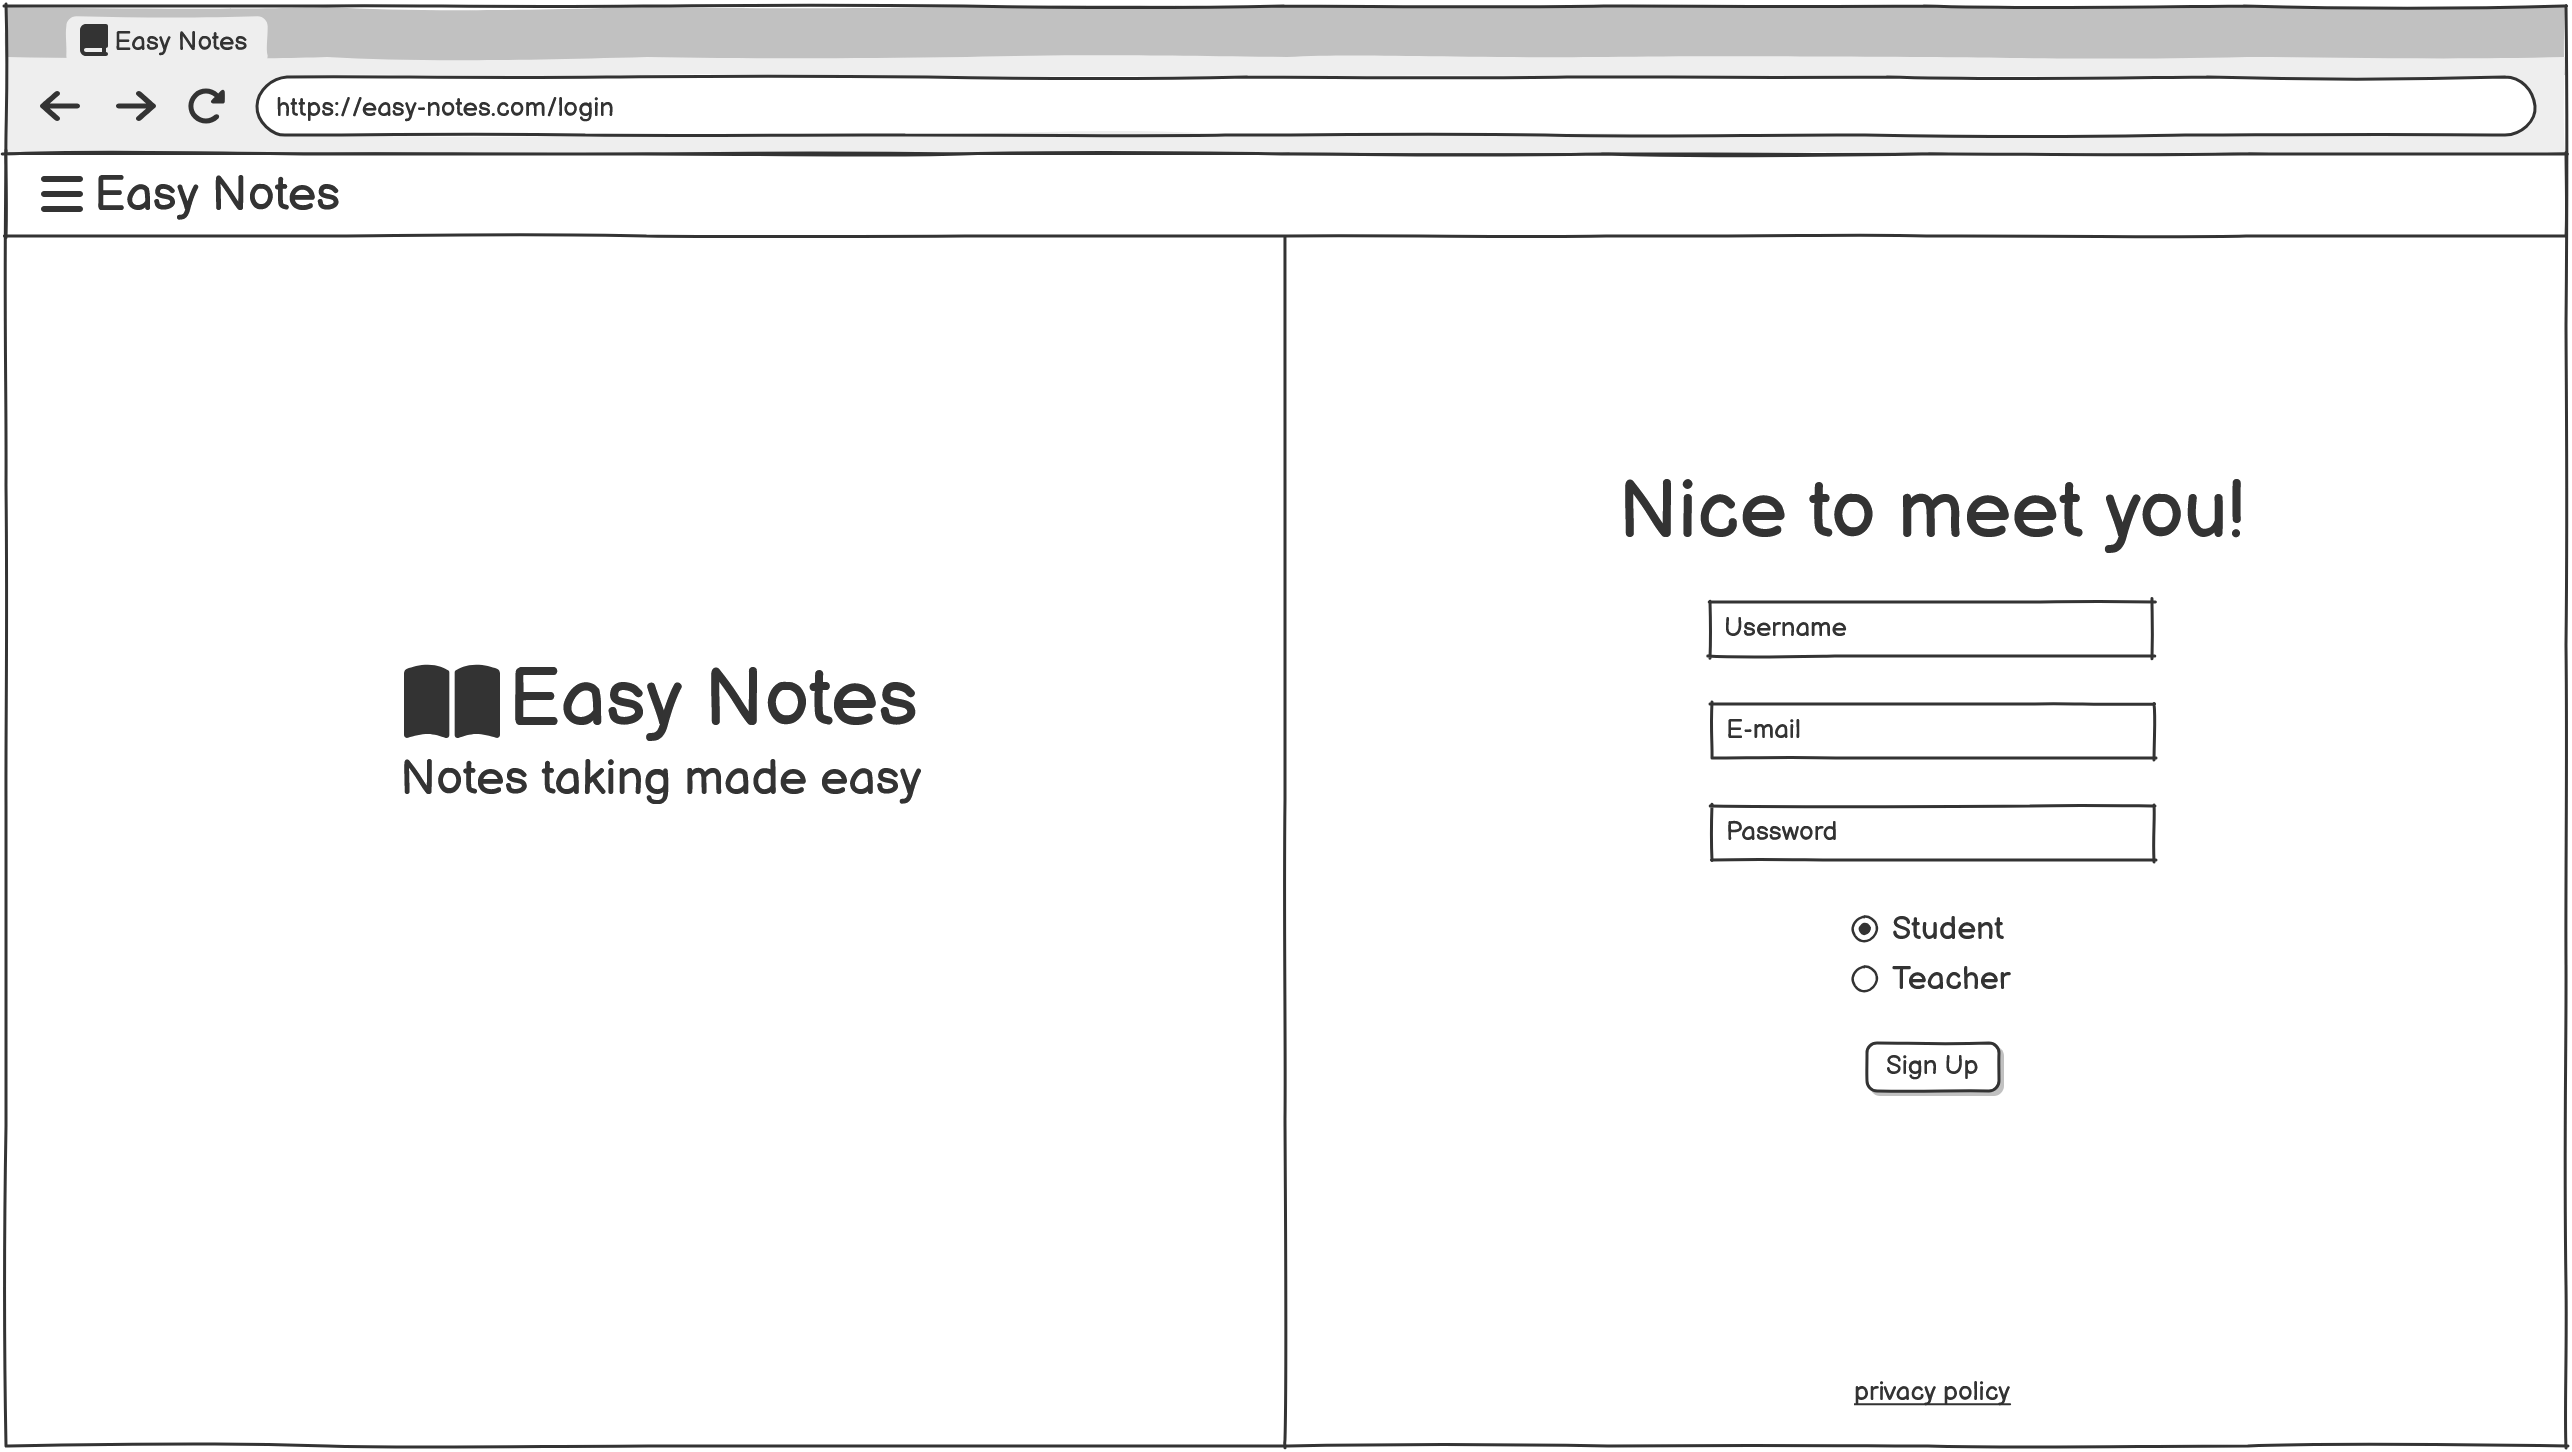
\includegraphics[width=1\textwidth]{mockup/Signin.png}
    \caption{Mockup pagina di registrazione}
    \label{fig:mockup_signin}
\end{figure}

Per concludere è degno di nota menzionare l'assenza di mockup mobile in quanto l'applicazione
è stata progettata esclusivamente per l'utilizzo su desktop e laptop, dove l'utente
può sfruttare al meglio lo schermo ampio per visualizzare sia le slide che le note
contemporaneamente. Infine, si può facilmente notare la consistenza stilistica della divisione
a metà delle pagine, questo proprio per mantenere l'effetto di un vero e proprio quaderno
digitale; la posizione delle pagine cerca, infatti, di seguire la direzione di lettura da sinistra verso
destra.
\newpage

\begin{figure}[h!]
    \centering
    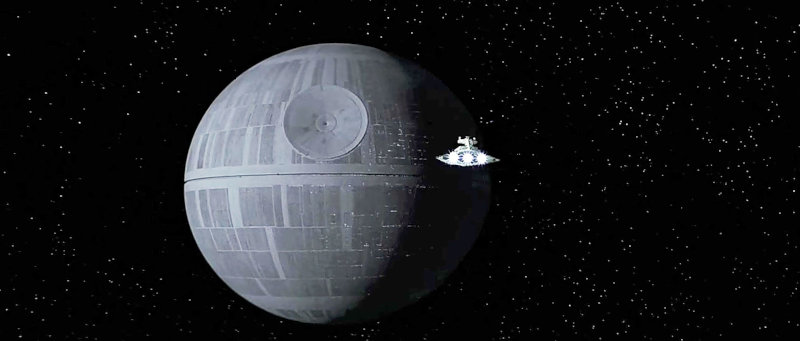
\includegraphics[scale=0.44]{figures/deathStar2.jpg}
    \caption{Death Star}
    \label{fig:deathstar}
\end{figure}

\section{Tecnologie}
Tecnologie adottate e motivazioni.

\section{Codice}
Solo aspetti rilevanti.

\section{Test}
Test effettuati sul codice e test con utenti.

\section{Deployment}
Rilascio, installazione e messa in funzione.


\section{Conclusioni}
Conclusioni

% TODO: remove this line when done
\citep{adams1995hitchhiker}

\bibliographystyle{plain}
\bibliography{references}
\end{document}
